%%%%%%%%%%%%%%%%%%%%%%%%%%%%%%%%%%%%%%%%%%%%%%%%%%%%%%%%%%%%%%%%%%%%%%%%%%%%%%%%%%%%%%
% Key Concept III       
%%%%%%%%%%%%%%%%%%%%%%%%%%%%%%%%%%%%%%%%%%%%%%%%%%%%%%%%%%%%%%%%%%%%%%%%%%%%%%%%%%%%%%
\section{Key Concept III \tiny Diskreter Ersatz für elektrische Signale}

\begin{tabular}{l|l}
	\multicolumn{2}{l}{\textbf{use.std\_logic\_1164.all} enthält folgende 2 Datentype}  \\
	std\_logic														& std\_ulogic \\
	\hline
	$\cdot$ solved logic											& $\cdot$ unsolved logic\\
	$\cdot$ erlaubt mehrere Treiber an einem Signal. Siehe Tabelle	& $\cdot$ erlaubt auch mehrere Treiber es darf aber nur einer aktiv sein \\
	$\rightarrow$ Kurzschluss Gefahr!								& $\rightarrow$ Kein Kurzschluss möglich  \\
	$\cdot$ Subklasse von std\_ulogic								& $\cdot$ erkennt in der Sim. nicht initialisierte Signale {\tiny bezeichnet sie als "`U"'}\\
	$\cdot$ erlaubt Modellierung von Schwachen Signalen (L und H)	& $\cdot$ erlaubt Modellierung von Schwachen Signalen (L und H)\\
	$\cdot$ erlaubt DONT'CARES (Signalwert '-')						& $\cdot$ erlaubt DONT'CARES (Signalwert '-')	\\
	$\cdot$ erlaubt bidirektionale Busse							& $\cdot$ nur einfache Busse erlaubt\\
	$\cdot$ grosser Simulationsaufwand								& $\cdot$ kleinerer Simulationsaufwand als std\_logic\\
	$\cdot$ Vektorform: std\_logic\_vector							& $\cdot$ Vektorform: std\_ulogic\_vector\\
\end{tabular}

\begin{minipage}{0.5\textwidth}
	\subsection{Busse}
	\begin{tabular}{l}
		$\cdot$ Master bestimmt welcher Slave spricht \\
		$\cdot$ Alle Teilnehmer (Slaves) können den Bus jederzeit abhören \\
		$\cdot$ Unaktive Treiber auf "`Z"' um den Datenverkehr nicht zu stören \\
		$\cdot$ Beschreibung des Zeitlichen Verhaltens  \\
		$\cdot$ Parametisierbarkeit von Modellen \\
	\end{tabular}
	\begin{minipage}{0.5\textwidth}
		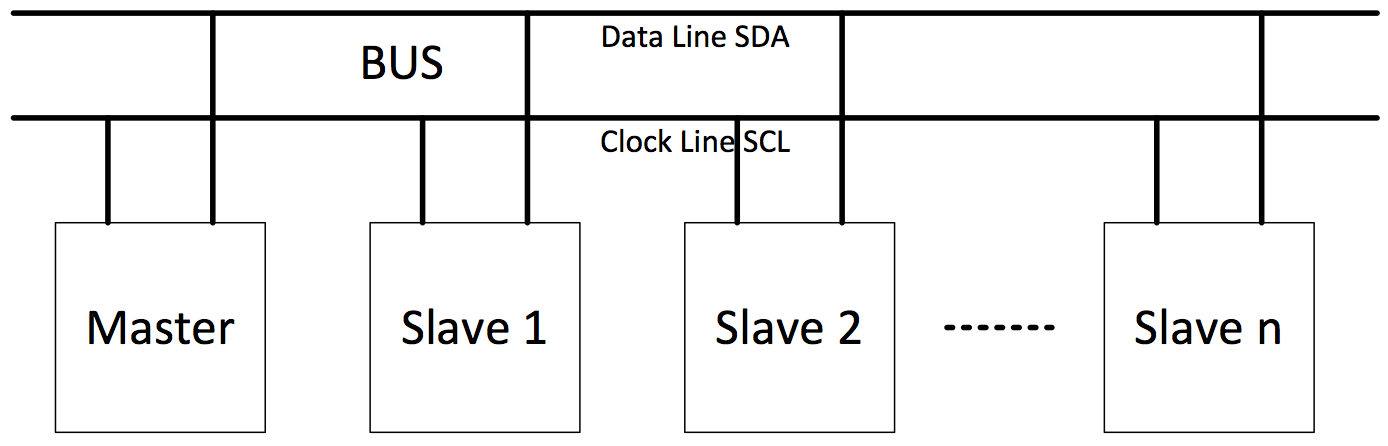
\includegraphics[width=\textwidth]{./bilder/Bus1}
	\end{minipage}
	\begin{minipage}{0.4\textwidth}
		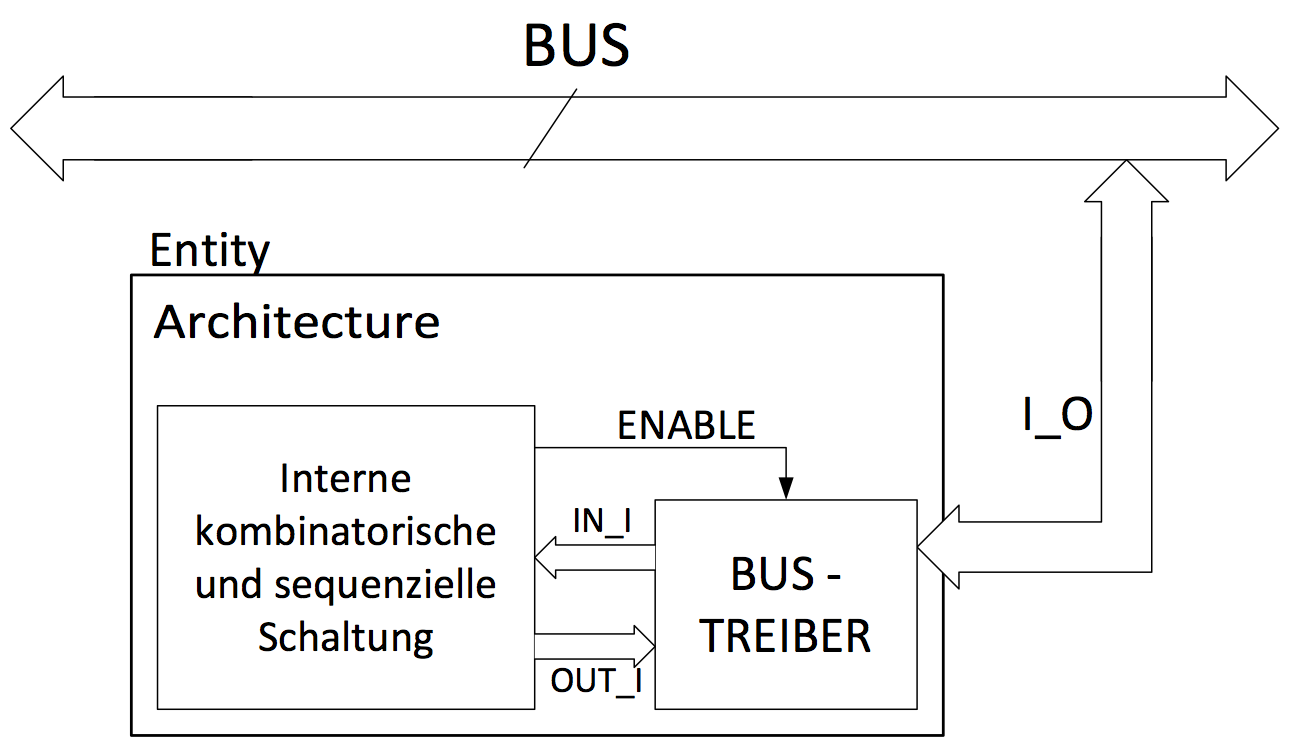
\includegraphics[width=\textwidth]{./bilder/Bus2}
	\end{minipage}
	\subsection{Codierungsempfehlung}
\end{minipage}
\begin{minipage}{0.5\textwidth}
	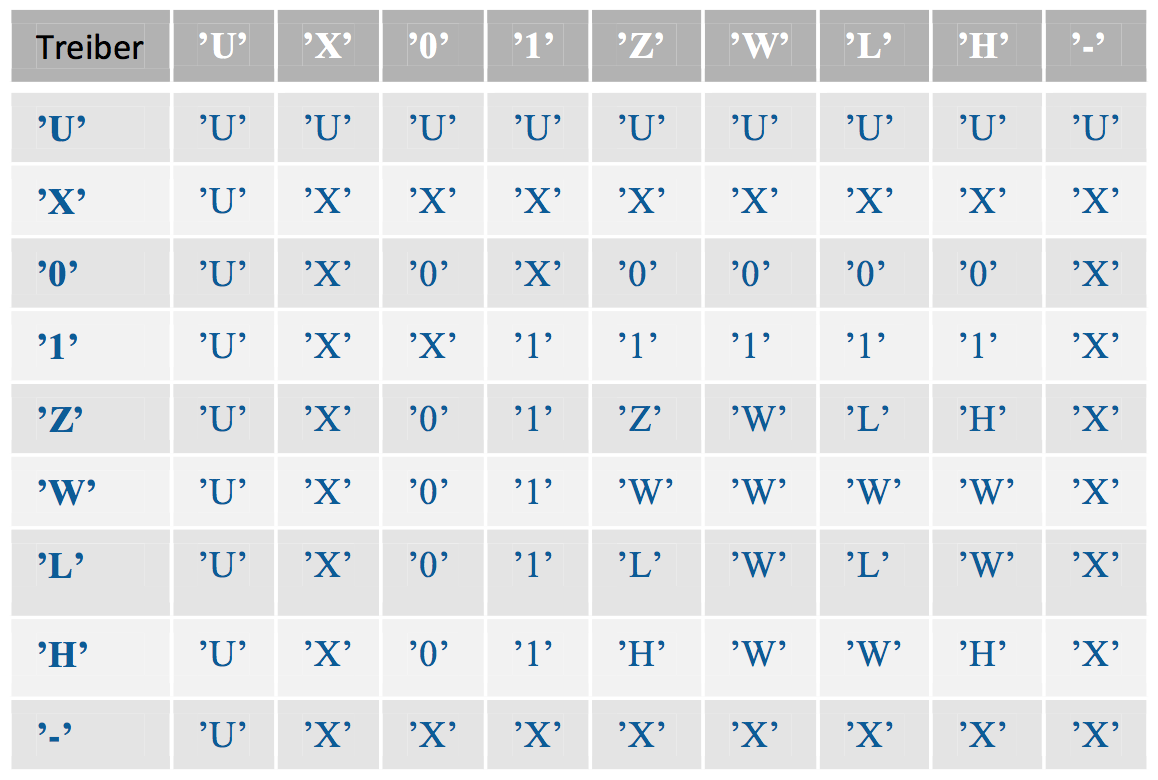
\includegraphics[width=\textwidth]{./bilder/Treiber}
\end{minipage}

Falls immer möglich (in den Übungen) std\_ulogic verwenden, obwohl in der Praxis std\_logic verbreitet ist. std\_logic ist eine Unterklasse von std\_ulogic und damit kompatibel, was aber nicht andersrum gilt! std\_logic\_vektor ist trotz Unterklasse erst seit 2008 mit std\_ulogic\_vektor kompatibel (dieser neuer STD ist noch nicht weit verbereitet!).